\documentclass[final]{beamer}
\mode<presentation> {\usetheme{Berlin}}

\usepackage{graphicx,ksu,url}
\usepackage{times}
\usepackage{amsmath,amssymb,amsfonts}
\usepackage[english]{babel}
\usepackage{standalone}
\usepackage{booktabs} % nice rules (thick lines) for tables
\usepackage[]{algorithm2e}
\usepackage{microtype} % improves typography for PDF
% Set your poster size here
\usepackage[orientation=por­trait,size=custom,width=91.44,height=121.92,scale=1,debug]{beamerposter}  % e.g. custom size poster, 36in(W) x 48in(H), converted to cm

% Add some information about your poster here
\title{Enhancements to the Discrete Generalized Multigroup Method}
\author[Reed, Roberts]{\vspace{1cm}R.L. Reed, J.A. Roberts}
\institute[Kansas State University]{Department of Mechanical and Nuclear Engineering, Kansas State University, Manhattan, KS 66506, USA}
\date[Dec. 2018]{Victor Menezes Convention Center, IIT Bombay, India}

% The real stuff goes in this block
\begin{document}
  \begin{frame}{} 
    % Begin block that spans the whole poster
%     \begin{block}{\large Fontsizes}
%       \centering
%       {\tiny tiny}\par
%       {\scriptsize scriptsize}\par
%       {\footnotesize footnotesize}\par
%       {\normalsize normalsize}\par
%       {\large large}\par
%       {\Large Large}\par
%       {\LARGE LARGE}\par
%       {\veryHuge veryHuge}\par
%       {\VeryHuge VeryHuge}\par
%       {\VERYHuge VERYHuge}\par
%     \end{block}
    % Add some space
%     \vfill
    
    % Split the poster into two columns
    % BEGIN columns
    \begin{columns}[t]
        % Left column
        % BEGIN column
        \begin{column}{.32\linewidth}
            \begin{block}{The Discrete Generalized Multigroup (DGM) Method}
                \begin{itemize}
                    \item The DGM method is a way to treat the energy variable in a numerical simulation \cite{zhu_discrete_2010}.
                    \item The method can work in conjunction with other schemes designed to treat the spatial and angular dependence.
                    \item DGM uses an orthogonal basis to collapse the group structure while preserving much of the accuracy \cite{reed2019effectiveness}.
                    \item The original method suffers from high memory costs since the angular flux must be stored \cite{gibson_stability_2014}.
                    \item Present work explores several incremental improvements, which may provide a way to use DGM for systematic generation of broad-group cross sections with implicit, fine-group features
                \end{itemize}
            \end{block}
            \vfill
            \begin{block}{Basis Sets}
                The first three vectors within each coarse group for the 238-group structure for the POD basis using snapshots of UO$_2$ pin combined with MOX pin snapshots.
                Note that DGM requires that the zeroth order basis be the flat vector to decouple the higher order moments.
                The vectors are orthonormalized over each coarse group region.
                The 238 fine-groups have been collapsed to 23 coarse-groups.
                \begin{figure}[htb]
                    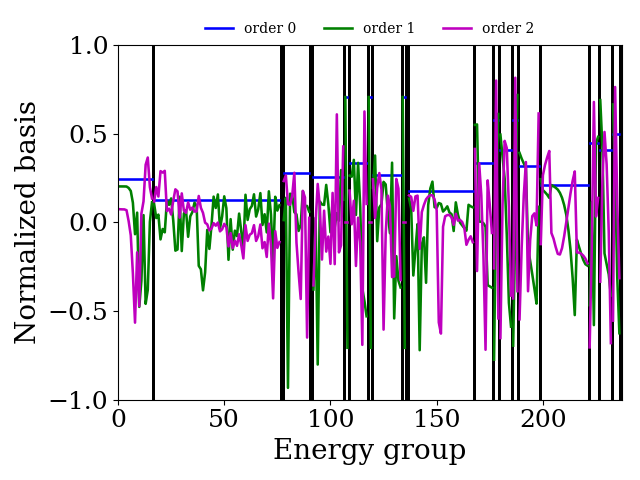
\includegraphics[scale=1.0, width=0.9\columnwidth]{klt_combine_contig_mean_238g}
                \end{figure}
            \end{block}
            % BEGIN block
            \begin{block}{The Discrete Generalized Multigroup (DGM) Equations}
                The DGM equations look similar to the multigroup form of the transport equations.
                In fact, the zeroth order equation is equivalent to the standard multigroup approximation.
                Note the presence of the $\delta$ term, which contains the angular dependence of the total cross section.
                % BEGIN equation
                \begin{equation*}
                    \begin{split}
                        \hat{\Omega} \cdot \nabla & \psi_{G,i}(\vec{r},\hat{\Omega}) 
                        + \Sigma^t_{G,0}(\vec{r}) \psi_{G,i}(\vec{r},\hat{\Omega})
                        + \delta_{G,i}(\vec{r}, \hat{\Omega}) \psi_{G,0}(\vec{r},\hat{\Omega}) \\
                        &= \frac{1}{4\pi} \sum^{N_G}_{G'=1} \Sigma^s_{G\leftarrow G',i}(\vec{r}) \phi_{G',0}(\vec{r})
                        + \frac{\chi_{G,i}}{4\pi k} \sum^{N_G}_{G'=1} \nu\Sigma^f_{G'}(\vec{r}) \phi_{G',0}(\vec{r})
                    \end{split}
                \end{equation*}
                % END equation
                where the coarse-group cross sections are defined as follows:
                \begin{equation*}
                    \Sigma^t_{G,0}(\vec{r}) 
                    = \frac{\sum\limits_{g\in G} \Sigma^t_{g}(\vec{r}) \phi_g(\vec{r})} 
                        {\sum\limits_{g\in G} \phi_g(\vec{r}) }
                    \quad\text{}\quad
                    \nu\Sigma^f_{G}(\vec{r}) 
                    = \frac{\sum\limits_{g\in G} P^G_{ig} \nu\Sigma^f_{g}(\vec{r}) \phi_{g}(\vec{r}) }
                        {\sum\limits_{g\in G} \phi_g(\vec{r}) }
                \end{equation*} 
                \begin{equation*}
                    \delta_{G,i}(\vec{r}, \hat{\Omega}) 
                    = \frac{\sum\limits_{g\in G} P^G_{ig} \left(\Sigma^t_{g}(\vec{r}) - \Sigma^t_{G,0}(\vec{r}) \right) \psi_g(\vec{r},\hat{\Omega})}
                        {\psi_{G,0}(\vec{r}, \hat{\Omega})}
                \end{equation*}
                \begin{equation*}
                    \Sigma^s_{G\gets G', i}(\vec{r}) 
                    = \frac{\sum\limits_{g\in G} P^G_{ig} \sum\limits_{g'\in G'} \Sigma^s_{g\gets g'}(\vec{r}) \phi_{g'}(\vec{r}) }
                        {\sum\limits_{g'\in G} \phi_{g'}(\vec{r}) }
                \end{equation*} 
                \begin{equation*}
                    \xi_{G,i} = \sum_{g\in G} P^G_{ig} \chi_g
                \end{equation*}
            \end{block}
            % END block
            % BEGIN block
            \begin{block}{Improvement 1 - Remove dependence on fine-group information}
                % BEGIN itemize
                \begin{itemize}
                    \item We want an algorithm that only uses the fine-group data once
                    \item To do so, redefine the cross sections in terms of flux moments to yield
                    \begin{equation*}
                        \Sigma^t_{c, G, 0} 
                        = \frac{\sum\limits_{j=1}^{N_j}\phi_{c,G,0,j}\Sigma^{t*}_{c, G, 0, j}}{\phi_{c,G,0,0}}
                        \quad\text{}\quad
                        \nu\Sigma^f_{c,G'}
                        = \frac{\sum\limits_{j=1}^{N_j}\phi_{c,G',0,j}\nu\Sigma^{f*}_{c,G',j}}{\phi_{c, G', 0, 0}}
                    \end{equation*}
                    \begin{equation*}
                        \delta_{c,a,G,i}=\frac{\sum_{j=1}^{N_j}\psi_{c,a,G,j}\Sigma^{t*}_{c, G, i, j}}{\psi_{c,a,G,0}} - \Sigma^t_{c, G, 0}\frac{\psi_{c,a,G,i}}{\psi_{c,a,G,0}}
                    \end{equation*}
                    \begin{equation*}
                        \Sigma_{c,G\leftarrow G',l,i}^s
                        = \frac{\sum_{j=1}^{N_j}\phi_{c,G',l,j}\Sigma_{c,G\leftarrow G',l,i,j}^{s*}}{\phi_{c,G,l,0}}
                    \end{equation*}
                    where
                    % BEGIN equation
                    \begin{equation*}
                        \begin{split}
                            \Sigma^{t*}_{c, G, i, j} &= \sum_{g=1}^{N_g^{G}}P_{ig}^G\Sigma^t_{c, g}P_{jg}^G\\
                            \nu\Sigma^{f,*}_{c,G',j} &= \sum_{g'=1}^{N_{g}^{G'}}P_{0g'}^{G'}\nu\Sigma^f_{c, g'} P_{jg'}^{G'}\\
                            \Sigma_{c,G\leftarrow G',l,i,j}^{s*} &= \sum_{g=1}^{N_g^{G}}P_{ig}^G\sum_{g'=1}^{N_g^{G'}}\Sigma^s_{c, g\leftarrow g',l}P_{jg'}^{G'}
                        \end{split}
                    \end{equation*}
                    % END equation
                    \item These new definitions must still be recomputed every iteration
                    \item The moment computations no longer use fine-group data
                \end{itemize}
                % END itemize
            \end{block}
            % END block
        \end{column}
        % END column
      
        % Center column
        \begin{column}{0.32\linewidth}
            \begin{block}{Old Algorithm}
                \DontPrintSemicolon
                \begin{algorithm}[H]
                    \KwIn{cell and material properties, basis vectors}
                    Compute $\chi$ and $Q$ moments\;
                    Guess the initial, fine-group flux\;
                    \While{not converged}{
                        Compute flux moments\;
                        Compute cross-section moments\;
                        Solve zeroth-order equations ($i=0$)\;
                        Update the eigenvalue\;
                        \For{all moments $i > 0$}{
                            Solve $i$th-order equation\;
                        }
                        Reconstruct fine-group flux\;
                    }
                \end{algorithm}
            \end{block}
            \vspace{0.55eX}
            \begin{block}{The Test Problem}
                Depiction of the 10-pin problem. 
                Each fuel section (UO$_2$/MOX) used 22 mesh cells, and each moderator section (blue) used 3 mesh cells.
                \begin{figure}[htb]
                    \includestandalone[mode=buildnew, width=\columnwidth]{10pin}
                \end{figure}
                The DGM method was implemented into a 1-D discrete ordinates code, which used the diamond difference approximation and 8 angles per half space.
            \end{block}
            \vspace{0.55eX}
            \begin{block}{Eigenvalue error for DGM method with truncation}
                Comparison of various basis sets used for the DGM method.
                Using DGM, a 1\% error in the eigenvalue may be reached using approximately 58 degrees of freedom for a 238-group problem.
                \begin{figure}[H]
                    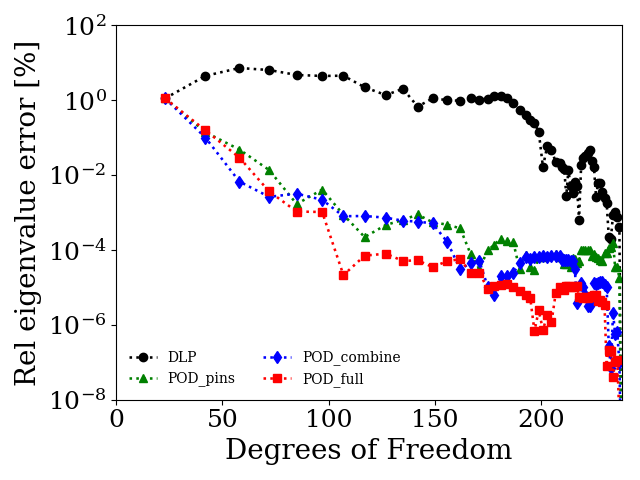
\includegraphics[scale=1.0, width=0.9\columnwidth]{k_error_238_h0}
                \end{figure}
                Note that at 238 degrees of freedom, all basis sets converge to within tolerance to the reference discrete ordinates solution (computed without DGM).
            \end{block}
            \vspace{0.55eX}
            \begin{block}{Improvement 2 - Approximate the angular flux}
                \begin{itemize}
                \item The definition for $\delta_{G,i}(\vec{r}, \hat{\Omega})$ depends on the angular flux
                \item This leads to a large memory footprint
                \item We can approximate the angular flux using a Legendre expansion
                \begin{equation*}
                    \psi_{g}(\vec{r}, \hat{\Omega})=\sum_{l=0}^\infty P_l(\hat{\Omega})\phi_{g, l}(\vec{r})
                \end{equation*}
                \item In this work, we consider both a zeroth and a first order expansion
                \item The definition for $\delta_{G,i}(\vec{r}, \hat{\Omega})$ now becomes
                \begin{equation*}
                    \delta_{G,i}(\vec{r}, \hat{\Omega}) 
                    = \frac{\sum\limits_{g\in G} P^G_{ig} \left(\Sigma^t_{g}(\vec{r}) - \Sigma^t_{G,0}(\vec{r}) \right) \sum\limits_{l=0}^{N_l} P_l(\hat{\Omega})\phi_{g, l}(\vec{r})}
                        {\sum\limits_{l=0}^{N_l} P_l(\hat{\Omega})\sum\limits_{g\in G} \phi_{g, l}(\vec{r})}
                \end{equation*}
                \end{itemize}
            \end{block}
            \vspace{0.55eX}
            \begin{block}{Improvement 3 - Spatially homogenize the cross sections}
                \begin{itemize}
                    \item The definitions for the cross section moments are functions of the flux
                    \item Since the flux is spatially dependent, the moments are as well
                    \item Thus, cross section data must be stored for each cell even if the cross sections are not normally spatially dependent
                    \item We spatially homogenize the moments using flux weighted averaging
                    \item The process is similar for all cross section moments
                    \item Take for example the total cross section moments
                    \begin{equation*}
                        \Sigma^t_{G,0}(R) =
                        \frac{\sum\limits_{c\in R}\Sigma^t_{G,0}(c) \Delta_c \phi_{g}(c)}
                        {\sum\limits_{c\in R} \Delta_c \phi_{g}(c)}
                    \end{equation*} 
                \end{itemize}
            \end{block}
            \vspace{0.55eX}
            \begin{block}{Acknowledgements}
                The work of the first author was supported by the Kansas State University Nuclear Research Fellowship Program, generously sponsored by the U.S. Nuclear Regulatory Commission (Grant NRC-HQ-84-14-G-0033).
            \end{block}
            \vspace{0.55eX}
        \end{column}

        
        % BEGIN column
        \begin{column}{.32\linewidth}
            \begin{block}{New Algorithm}
                \DontPrintSemicolon
                \begin{algorithm}[H]
                    \KwIn{cell and material properties, basis vectors}
                    Compute $\chi$ and $Q$ moments and expand fine-group cross-sections\;
                    Guess the initial, fine-group flux\;
                    Compute flux moments\;
                    \While{not converged}{
                        Compute coarse-group cross-section moments\;
                        Solve zeroth-order equation ($i=0$)\;
                        Update the eigenvalue\;
                        \For{all moments $i > 0$}{
                            Solve $i$th-order equation\;
                        }
                    }
                    Reconstruct fine-group flux\;
                \end{algorithm}
            \end{block}
            \vspace{0.1eX}
            \begin{block}{Improvement Cases}
                To evaluate the performance of the method, we define several cases
                \begin{itemize}
                    \item Case 1: Assume flat angular flux (Improvement 2)
                    \item Case 2: Assume linear angular flux (Improvement 2)
                    \item Case 3: Spatial homogenization (Improvement 3)
                    \item Case 4: Both linear angular flux and spatial homogenization
                \end{itemize}
                We also explored how these cases behave in both the full order problem and the truncated case.
            \end{block}
            \vspace{0.1eX}
            \begin{block}{Scalar flux for full problem for group 0}
                Fine-group scalar flux for the fastest energy group reconstructed using the DGM method.
                Improvement 3 causes slight deviation from the reference solution, whereas improvement 2 leads to a larger effect.
                \begin{figure}[htb]
                    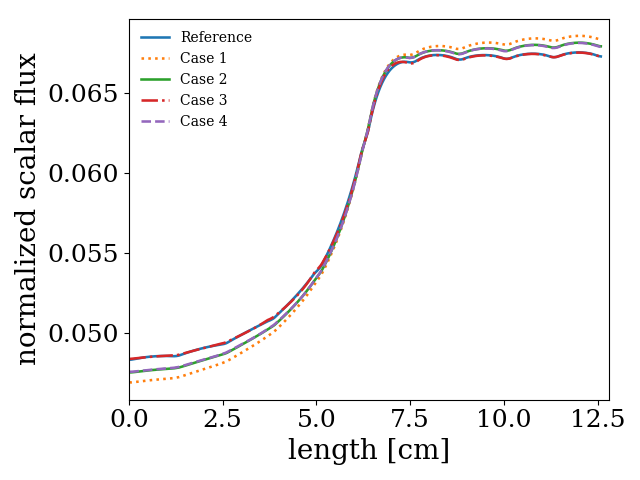
\includegraphics[scale=1.0, width=0.9\columnwidth]{phi_g0_o59}
                \end{figure}
            \end{block}
            \vspace{0.1eX}
            \begin{block}{Case results for full problem compared to reference}
                \centering
                The following table compares the DGM improvements to a discrete ordinates solution with no DGM.
                Note all data are relative percent error except for the first column, which are the reference values.
                \vspace{2eX}
                
                \begin{tabular}{c|r|r|r|r|r}
                & Full-Ref & Full-(1)  & Full-(2) & Full-(3) & Full-(4)\\
                \hline
                $k_{\text{eff}}$& 1.122 & -0.038\% & -0.036\% &  0.040\% & -0.021\%\\
                \hline
                Cell 1&  0.939 & -0.471\% & -0.288\% & -0.096\% & -0.310\%\\
                Cell 2&  0.917 & -0.456\% & -0.279\% & -0.099\% & -0.303\%\\
                Cell 3&  0.866 & -0.425\% & -0.261\% & -0.104\% & -0.286\%\\
                Cell 4&  0.770 & -0.380\% & -0.237\% & -0.107\% & -0.256\%\\
                Cell 5&  0.598 & -0.335\% & -0.218\% & -0.088\% & -0.204\%\\
                Cell 6&  1.736 &  0.084\% & -0.014\% &  0.280\% &  0.112\%\\
                Cell 7&  1.151 &  0.447\% &  0.301\% & -0.133\% &  0.193\%\\
                Cell 8&  1.031 &  0.400\% &  0.277\% &  0.027\% &  0.268\%\\
                Cell 9&  1.000 &  0.344\% &  0.241\% &  0.024\% &  0.235\%\\
                Cell 10& 0.992 &  0.308\% &  0.218\% &  0.020\% &  0.210\%\\
                \hline
                \end{tabular}
                
            \end{block}
            \vspace{0.1eX}
            \begin{block}{Case results for truncated problem compared to reference}
                \centering
                The following table compares the DGM improvements to a discrete ordinates solution with no DGM.
                Note all data are relative percent error except for the first column, which are the reference values.
                \vspace{2eX}
                
                \begin{tabular}{c|r|r|r|r|r|r}
                & Full-Ref & Trun.-Ref & Trun.-(1) &  Trun.-(2)  &  Trun.-(3)  &  Trun.-(4)  \\
                \hline
                $k_{\text{eff}}$& 1.122 &  0.007\% & -0.028\% & -0.019\% &  0.014\% & -0.011\%\\
                \hline
                Cell 1&  0.939 & -0.078\% & -0.612\% & -0.418\% & -0.125\% & -0.435\%\\
                Cell 2&  0.917 & -0.091\% & -0.601\% & -0.416\% & -0.143\% & -0.436\%\\
                Cell 3&  0.866 & -0.126\% & -0.586\% & -0.419\% & -0.183\% & -0.442\%\\
                Cell 4&  0.770 & -0.203\% & -0.586\% & -0.450\% & -0.266\% & -0.473\%\\
                Cell 5&  0.598 & -0.405\% & -0.678\% & -0.586\% & -0.456\% & -0.590\%\\
                Cell 6&  1.736 &  0.392\% &  0.459\% &  0.405\% &  0.526\% &  0.474\%\\
                Cell 7&  1.151 &  0.004\% &  0.423\% &  0.280\% & -0.033\% &  0.245\%\\
                Cell 8&  1.031 & -0.048\% &  0.382\% &  0.241\% & -0.036\% &  0.241\%\\
                Cell 9&  1.000 &  0.005\% &  0.407\% &  0.277\% &  0.015\% &  0.276\%\\
                Cell 10& 0.992 &  0.025\% &  0.407\% &  0.285\% &  0.032\% &  0.280\%\\
                \hline
                \end{tabular}
            \end{block}
            \vspace{0.1eX}
            \begin{block}{\large References} 
                \bibliographystyle{ans}
                \small
                \bibliography{references}
            \end{block}
        \end{column}
        % END column
    \end{columns}
    % END columns
  \end{frame}
\end{document}